
\newpage\section{Orbit Determination and Parameter Estimation}
%%%%%%%%%%%%%%%%%%%%%%%%%%%%%%%%%%%%%%%%%%%%%%%%%%%%%%%%%%%%%%%%%%%%%%%%%%%%%%%%

%Preliminary orbit determination is useful in an initial determination of the
%orbital elements of a satellite's motion and can be carried out using two
%position vectors of the satellite relative to the observing ground station.

Predicting the state ($\bm{x}_t$) of a spacecraft given an initial condition
($\bm{x}_0$), and models which form the equations of motion of the satellite,
($\dot{\bm{x}}=f(t,\bm{x})$), is a straightforward task involving the solution
of an initial value problem (IVP) in the form of an ordinary differential
equation (ODE). However the inverse problem  is more involved, that is, given a
set of measurements ($\bm{z}$) resulting from the dynamical system, we would
like to estimate the trajectory of the satellite and the parameters describing
the dynamical models, described mathematically as:
\begin{equation}
    \bm{x}(t) =
    \begin{bmatrix}
        \bm{r}(t) \\
        \bm{v}(t) \\
        \bm{p} \\
        \bm{q} \\
    \end{bmatrix}.
\end{equation}
\begin{equation*}
    \begin{aligned}
        \textrm{where  }
            \bm{r}(t), \bm{v}(t) &= \text{the position and velocity of the spacecraft as a function of time,} \\
            \bm{p}               &= \text{the parameters describing the force models,} \\
            \bm{q}               &= \text{the parameters describing the measurement models.} \\
    \end{aligned}
\end{equation*}

The measurements made throughout the trajectory of the spacecraft at times
$t_1,...,t_n$ are described by $\bm{z}=[z_1,...,z_n]^T$, where each $z_i$ is
either defined as a function of the state of the spacecraft at time $t_i$, or
as a function of the state of the spacecraft at time $t_0$:
\begin{equation}
    z_i(t_i) = g_i(t_i, \bm{x}(t_i))+\epsilon_i = h_i(t_i, \bm{x}_0)+\epsilon_i.
\end{equation}
\begin{equation*}
    \begin{aligned}
        \textrm{where  }
            z_i &= \text{the i$^{th}$ empirical measurement, assumed to be a random variable,} \\
            g_i &= \text{the i$^{th}$ model measurement as a function time and instantaneous state,} \\
            h_i &= \text{the i$^{th}$ model measurement as a function time and initial state,} \\
            \epsilon_i &= \text{the i$^{th}$ residual, accounting for measurement errors.} \\
    \end{aligned}
\end{equation*}

The expressions of $h_i$ and $g_i$ can be used interchangeably in the
measurement model predictions, to account for the fact that the measurements are
often made at different times than the respective instantaneous states of the
spacecraft. This is done using variational equations, which are simulated to
obtain the state transition matrix $\bm{\Phi}(t_0, t)$ of the spacecraft, as
described in \autoref{sec:linearization}, which may be interpolated for any
arbitrary time within the temporal bounds of the ODE solution across
$t_i\in[t_0, t_f]$ \cite[p.~]{Montenbruck2000}, so that one may relate an
empirical $z_i$ at $\bm{x}(t_i)$ to $\bm{x}_0$ through $\bm{\Phi}(t_0,
t_i)^{-1}\bm{x}_0$. This effectively constrains the trajectory to the designed
IVP dynamical solution. Consequentially, the measurements concisely:
\begin{equation}
    \bm{z} = \bm{h}(\bm{x}_0) + \bm{\epsilon}.
\end{equation}


%\begin{figure}[h]
%    \centering
%    \def\svgwidth{0.95\linewidth}
%    % \input{graphics/drawing2.pdf_tex}
%    \import{graphics/}{trajectory_estimation.pdf_tex}
%    \caption{Definition of a general Body-centered inertial (BCI) reference frame.}
%    \label{fig:as}
%\end{figure}


%Furthermore, the accuracy of this solution can be
%traded off against the computational expense of the prediction.

%
%\begin{itemize}
%    \item Orbit of asteroid
%    \item Orbit of spacecraft
%    \item Rotation of asteroid (rate + principle axes)
%    \item Gravitational potential of asteroid
%\end{itemize}

%%%%%%%%%%%%%%%%%%%%%%%%%%%%%%%%%%%%%%%%%%%%%%%%%%%%%%%%%%%%%%%%%%%%%%%%%%%%%%%%
\subsection{Least Squares (batch estimation)}
%%%%%%%%%%%%%%%%%%%%%%%%%%%%%%%%%%%%%%%%%%%%%%%%%%%%%%%%%%%%%%%%%%%%%%%%%%%%%%%%

The least-squares method was officially discovered and published by Adrien-Marie
Legendre in their work ``\textit{Nouvelles methodes pour la determination des
orbites des cometes}”, published in 1805 \cite{nla.cat-vn866184}.

%%%%%%%%%%%%%%%%%%%%%%%%%%%%%%%%%%%%%%%%%%%%%%%%%%%%%%%%%%%%%%%%%%%%%%%%%%%%%%%%
\subsubsection{Weighted Least-Squares}
%%%%%%%%%%%%%%%%%%%%%%%%%%%%%%%%%%%%%%%%%%%%%%%%%%%%%%%%%%%%%%%%%%%%%%%%%%%%%%%%

The Weighted Least-Squares Estimation method is an application of the
Generalized Least-Squares (GLS) algorithm~\cite{Aitken1936}, which aims at
estimating unknown parameters ($\bm{\beta}$) in a linear regression model,
given a set of observations ($\bm{z}$), where there is a certain degree of
correlation ($\bm{W}$) between the residuals ($\bm{\epsilon}$) in the
regression model. It is usually written as:
\begin{equation}
    \begin{aligned}
        \bm{z}&=\bm{A}\bm{\beta}+\bm{\epsilon},\\
        \;\;\;\gls{E}{}[\bm{\epsilon}|\bm{A}]&=\bm{0},\\
        \;\;\;\text{Cov}(\bm{\epsilon}|\bm{A})&=\bm{W}.
    \end{aligned}
\label{eq:linear-regression}
\end{equation}

The residual vector is defined as $\bm{\rho}=\bm{z}-\bm{A}\hat{\bm{\beta}}$. The
Weighted Least-Squares estimate ($\bm{\hat{\beta}}$) is unbiased, consistent and
efficient, and obtained through minimising $\bm{\rho}^T\bm{W}^{-1}\bm{\rho}$.
The estimate is given, without derivation, by:

%where $\bm{\hat{\beta}}$ is an

\begin{equation}
    \begin{aligned}
        \bm{\hat{\beta}} &= (\bm{A}^T\bm{W}^{-1}\bm{A})^{-1}\bm{A}^T\bm{W}^{-1}\bm{z}, \\
        \bm{\hat{\beta}} &= \text{argmin}(\bm{\rho}^T\bm{W}^{-1}\bm{\rho}), \\
        \mathbb{E}[\bm{\hat{\beta}}] &= \bm{\beta}, \\
        \text{Cov}[\bm{\hat{\beta}}|\bm{A}] &= (\bm{A}^T\bm{W}^{-1}\bm{A})^{-1}. \\
    \end{aligned}
\end{equation}

%%%%%%%%%%%%%%%%%%%%%%%%%%%%%%%%%%%%%%%%%%%%%%%%%%%%%%%%%%%%%%%%%%%%%%%%%%%%%%%%
\subsubsection{Non-linear Least Squares}
%%%%%%%%%%%%%%%%%%%%%%%%%%%%%%%%%%%%%%%%%%%%%%%%%%%%%%%%%%%%%%%%%%%%%%%%%%%%%%%%

The problem arises when considering the highly non-linear modelled measurements
$\bm{h}(\bm{x}_0)$ cannot be described by the linear relation in
\autoref{eq:linear-regression}. For this reason, the model is linearized by
approximation to a first-order Taylor polynomial expansion about $\bm{\beta}$,
for a step size $\Delta\bm{\beta}$. The resulting linearized model is:
\begin{equation}
    \begin{aligned}
        \bm{z}                              &=        f(\bm{\beta}) + \bm{\epsilon}                                                              \\
        f(\bm{\beta}+\Delta\bm{\beta}) &\approx  f(\bm{\beta}) + \frac{\partial{f(\bm{\beta})}}{\partial{\bm{\beta}}}\Delta\bm{\beta}  \\
    \end{aligned}
\end{equation}

\begin{equation}
    \begin{aligned}
        \bm{\rho} &= f(\bm{\beta}) - f(\bm{\beta}^*)  + \frac{\partial{f(\bm{\beta})}}{\partial{\bm{\beta}}}\Delta\bm{\beta}  \\
        \bm{\rho} &= \Delta\bm{z}  + \bm{H}\Delta\bm{\beta}  \\
    \end{aligned}
\end{equation}

\begin{equation}
    \begin{aligned}
        \Delta\hat{\bm{\beta}} &= (\bm{H}^T\bm{H})^{-1}\bm{H}^T\Delta\bm{z}  \\
        \hat{\bm{\beta}}^*     &= \hat{\bm{\beta}} + \Delta\hat{\bm{\beta}}  \\
    \end{aligned}
\end{equation}

\begin{equation}
    \left|\frac {\Delta\hat{\bm{\beta}}}{\hat{\bm{\beta}}}\right|<0.001,\qquad j=1,\dots ,n.
\end{equation}

\cite{Kelley1999}

%%%%%%%%%%%%%%%%%%%%%%%%%%%%%%%%%%%%%%%%%%%%%%%%%%%%%%%%%%%%%%%%%%%%%%%%%%%%%%%%
\subsection{Kalman Filter}
%%%%%%%%%%%%%%%%%%%%%%%%%%%%%%%%%%%%%%%%%%%%%%%%%%%%%%%%%%%%%%%%%%%%%%%%%%%%%%%%

Without Western academia,
by Rudolf E. Kalman \cite{Kalman1960, Kalman1961} and Richard S. Bucy \cite{Kalman1961}


\def\predictstate{\vbox{
\begin{equation}
   \hat{\bm{x}}_{i|i-1} = \bm{\Phi}_i\,\hat{\bm{x}}_{i-1|i-1} + \bm{B}_i\,\bm{u}_{i}
\end{equation}
}}

\def\predictcovariance{\vbox{
\begin{equation}
   \bm{P}_{i|i-1} = \bm{\Phi}_i\bm{P}_{i-1|i-1}\bm{\Phi}_i^T+\bm{Q}_i
\end{equation}
}}

\def\prefitresidual{\vbox{
\begin{equation}
   \bm{\rho}_i = \bm{z}_i - \bm{H}_i\hat{\bm{x}}_{i|i+1}
\end{equation}
}}

\def\prefitcovariance{\vbox{
\begin{equation}
   \bm{S}_i = \bm{H}_i\bm{P}_{i|i-1}\bm{H}_i^T + \bm{R}_i
\end{equation}
}}

\def\kalmangain{\vbox{
\begin{equation}
   \bm{K}_i = \bm{P}_{i|i-1}\bm{H}_i^T\bm{S}_i^{-1}
\end{equation}}}

\def\updatedstate{\vbox{
\begin{equation}
   \hat{\bm{x}}_{i|i} = \hat{\bm{x}}_{i|i-1} + \bm{K}_i\bm{\rho}_i
\end{equation}}}

\def\updatedcovariance{\vbox{
\begin{equation}
   \bm{P}_{i|i} = (\bm{I} - \bm{K}_i\bm{H}_i)\bm{P}_{i|i-1}
\end{equation}
}}

\def\postfitresidual{\vbox{
\begin{equation}
   \bm{\rho}_{i|i} = \bm{z}_i - \bm{H}_i\hat{\bm{x}}_{i|i}
\end{equation}
}}

\def\where{\vbox{
\begin{equation*}
   \begin{aligned}
       \text{where  }
        \bm{\Phi}_i &= \text{The state-transition matrix from }t_{t-1}\text{ to }t_i: \bm{\Phi}(t_i, t_{i-1}) \\
        \bm{B}      &= \text{Control Matrix} \\
        \bm{Q}      &= \text{Process Noise Covariance} \\
        \bm{R}      &= \text{Measurement Noise Covariance} \\
        \bm{H}      &= \text{Measurement Matrix} \\
        \bm{z}      &= \text{Measurement} \\
        \bm{u}      &= \text{Control} \\
        \bm{\rho}   &= \text{Residual} \\
        \bm{S}      &= \text{Pre-fit residual covariance} \\
        \bm{K}      &= \text{Kalman Gain} \\
        \bm{\hat{\bm{x}}} &= \text{Updated state} \\
        \bm{\bm{P}}    &= \text{Updated covariance} \\
        \bm{\bm{\rho}} &= \text{Post-fit residual} \\
   \end{aligned}
\end{equation*}
}}

\newpage\begin{table}[htp!]
\renewcommand{\arraystretch}{1.4}
\centering
\caption{
    \textbf{}
}
\label{tab:kalman-equations}
\begin{tabularx}{\textwidth}{l X}
\hline
\textbf{Description}                        & \textbf{Equation}      \\
\hline\hline
\multicolumn{2}{l}{\textbf{Prediction phase}}                        \\
\hline
Predicted (a priori) state estimate         & \predictstate          \\
Predicted (a priori) estimate covariance    & \predictcovariance     \\
\hline
\multicolumn{2}{l}{\textbf{Update phase}}                            \\
\hline
Innovation or measurement pre-fit residual  & \prefitresidual        \\
Innovation (or pre-fit residual) covariance & \prefitcovariance      \\
Optimal Kalman gain                         & \kalmangain            \\
Updated (a posteriori) state estimate       & \updatedstate          \\
Updated (a posteriori) estimate covariance  & \updatedcovariance     \\
Measurement post-fit residual               & \postfitresidual       \\
\hline
\multicolumn{2}{l}{\where}                                           \\
\hline\hline
\end{tabularx}
\end{table}

\subsubsection{Linearized Kalman Filter}

simplicity,
optimality, tractability and robustness

\begin{figure}[htp]
    \centering
    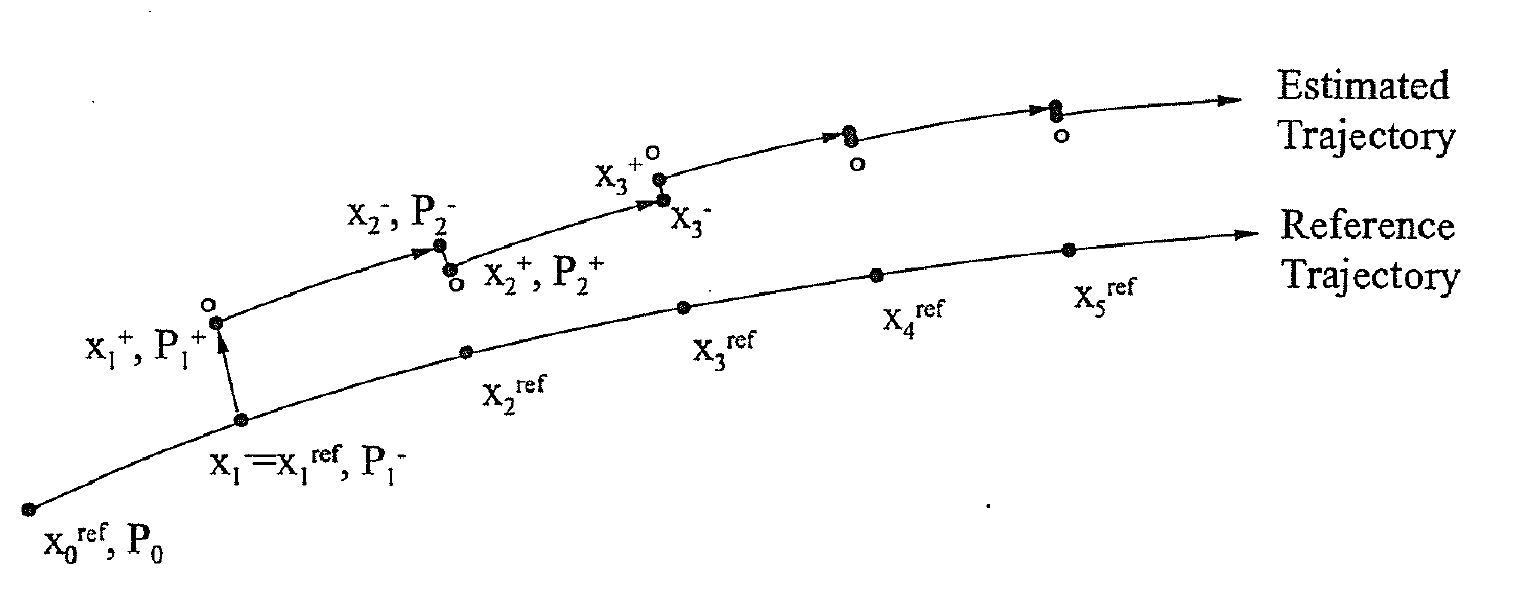
\includegraphics[width=0.8\linewidth]{graphics/lkf.PNG}
    \caption{CEKF flow diagram for process of tracking and data prediction including all equations \cite{3}.}
    \label{fig:LKF}
\end{figure}


\subsubsection{Extended Kalman Filter}

However, the application of the KF to nonlinear systems can be complex. The most common approach is the Extended Kalman Filter (EKF), which linearises all nonlinear models to apply the traditional linear Kalman filter. Although the EKF (in its many forms) is a widely used filtering strategy, over thirty years of experience with it has led to a consensus within the tracking and control community that it is challenging to implement, difficult to tune, and only reliable for systems which are almost linear on the time scale of the update intervals.

\begin{equation}
   \hat{\bm{x}}_{i}^- = f({\bm{x}}_{i-1}^+,\bm{u}_{i})
\end{equation}

\begin{equation}
   \bm{\rho}_i = \bm{z}_i - h(\hat{\bm{x}}_{i}^+)
\end{equation}

Although superior to Linearized Kalman Filtering in that the state propagation
is represented correctly by the non-linear system; the main drawback is that the
covariance is propagated through the linearised state transition matrix. This
results in the uncertainty of the system being non-representative of the true
non-linear system.

\begin{figure}[htp]
    \centering
    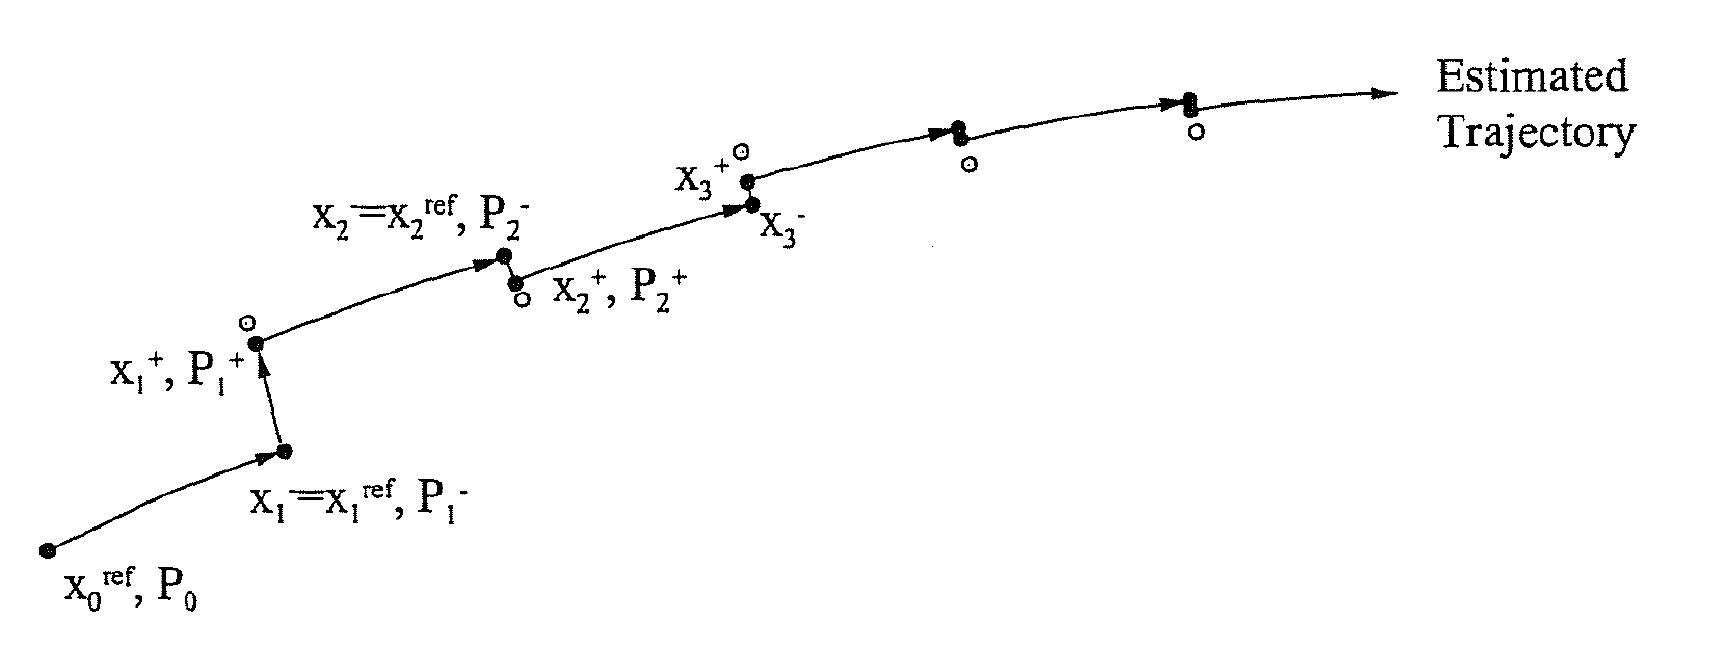
\includegraphics[width=0.8\linewidth]{graphics/ekf.PNG}
    \caption{CEKF flow diagram for process of tracking and data prediction including all equations \cite{3}.}
    \label{fig:LKF}
\end{figure}

\subsubsection{Unscented Kalman Filter}

First and second-order terms of the nonlinear system captured through the
addition of the unscented transform (UT).

Proposed by Julier and Uhlmann in 1997~\cite{Julier1997}

\cite{Wan2000, Wan2001}
In order to combat the first-order propagation of covariance, a set of sigma
points is chosen at each estimation step. These are chosen according to the
covariance of the current state estimate and are passed through the non-linear
system to produce weighted estimates of the mean state and its covariance.

\begin{equation}
    \begin{aligned}
        \hat{\bm{x}}_0 &= \mathbb{E}[\bm{x}_0]                                             \\
        \bm{P}_0       &= \mathbb{E}[(\bm{x}_0-\hat{\bm{x}}_0)(\bm{x}_0-\hat{\bm{x}}_0)^T] \\
    \end{aligned}
\end{equation}

\cite{Cheng2011}
The \textbf{sigma points} can be selected by

\begin{equation}
    \begin{aligned}
        L                   &= \text{dim}(\hat{\bm{x}})                                                      && \bm{x}\in{\gls{set:R}}^{L} \\
        \mathcal{X}_0       &= \hat{\bm{x}}_{i-1}^{+}                                                                                     \\
        \mathcal{X}_j       &= \hat{\bm{x}}_{i-1}^{+} + \sqrt{(L+\lambda)} \bm{A}_j                          && j=1,...,L                 \\
        \mathcal{X}_{L+j}   &= \hat{\bm{x}}_{i-1}^{+} - \sqrt{(L+\lambda)} \bm{A}_j                          && j=1,...,L                 \\
        W_0^{(m)}           &= \lambda(L-\lambda)                                                                                         \\
        W_0^{(c)}           &= \lambda(L-\lambda) + (1-\alpha^2 + \beta)                                                                  \\
        W_k^{(m)}           &= W_k^{(c)} = 1/\{2(L+\lambda)\}                                                && j=1,...,2L                \\
    \end{aligned}
\end{equation}
\begin{equation*}
    \begin{aligned}
    \text{where  }
        \lambda &= \alpha^2(L+\kappa)-L,\text{ a scaling parameter,} \\
        \alpha  &= \text{parameter determining spread of sigma points about }\hat{\bm{x}}\text{,} \\
        \kappa  &= \text{secondary scaling parameter, usually set to }0, \\
        \beta   &= \text{ parameter for incorporation of prior knowledge of }p(\hat{\bm{x}}).\\
    \end{aligned}
\end{equation*}

For Gaussian distributions, $\beta=2$ is an an optimal choice and often $\alpha$
is set to some small positive value (e.g. 1e-3) \cite{Wan2000}. The sigma points
are then propagated through the non-linear observation model,
\begin{equation}
    \mathcal{Z}_k  = h(\mathcal{X}_k)\,\,\,\,\,\,k=1,...,2L
\end{equation}

and the mean and covariance of $\bm{z}$ is approximated using the weighted
sample mean and covariance of the posterior sigma points,

\begin{equation}
    \begin{aligned}
        \bar{\bm{z}} & \approx \sum_{k=0}^{2L} W_k^{(m)}\mathcal{Z}_k                                                   \\
        \bm{P}_i     & \approx \sum_{k=0}^{2L} W_k^{(c)}\{\mathcal{Z}_k-\bar{\bm{z}}\}\{\mathcal{Z}_k-\bar{\bm{z}}\}^T +\bm{Q}_k. \\
    \end{aligned}
\end{equation}



\begin{equation}
   \bm{\rho}_i = \bm{z}_i - h(\bar{\bm{x}}_{i|i+1})
\end{equation}


% Notethatthismethoddifferssubstantiallyfromgeneral“sam-pling”methods(e.g.,Monte-Carlomethodssuchasparticlefilters[1])whichrequireordersofmagnitudemoresamplepointsinanattempttopropagateanaccurate(possiblynon-Gaussian)distributionofthestate.Thedeceptivelysim-pleapproachtakenwiththeUTresultsinapproximationsthatareaccuratetothethirdorderforGaussianinputsforallnonlinearities.Fornon-Gaussianinputs,approximationsareaccuratetoatleastthesecond-order,withtheaccuracyofthirdandhigherordermomentsdeterminedbythechoiceofand(See[4]foradetaileddiscussionoftheUT).

\begin{equation}
   \bm{\rho}_i = \bm{z}_i - h(\bar{\bm{x}}_{i|i+1})
\end{equation}

\begin{figure}[h]
    \centering
    \def\svgwidth{0.75\linewidth}
    \import{graphics/}{ukf.pdf_tex}
    \caption{Definition of a right-handed reference frame.}
    \label{fig:frames_rh}
\end{figure}

\subsubsection{Joint versus Dual Filtering}

In general, dual estimation methods are more computationally advantageous, and
joint estimation methods are more accurate \cite{Plett2005}.



%\noindent{}A CEKF consists of 3 main steps, namely: \textit{Initialisation (0)}, \textit{Prediction (1)} and \textit{Correction (2)}, where steps 1 \& 2 are iterated through $K-1$ times, where $K$ ($K\in\mathbb{Z}^+$) quantifies the number of Epochs.
%
%\begin{itemize}
%    \item \textbf{Step (0) Initialisation}: The \textit{a posteriori} estimate of the initial state ($\hat{x}_0^+$) is determined according to the expectation of the true value $x_0$. The initial state error covariance matrix is calculated according to the expectation of the covariance between $\hat{x}_0^+$ and $x_0$. Within the context of satellite tracking, a predefined $\hat{x}_0^+$ will be used throughout the CEKF analysis to analyse the performance as a result of the selection of hyper-parameters: $\bm{Q}_{k-1}$ and $\bm{R}_k$.
%    \item \textbf{Step (1) Prediction}: Project the state and its co-variance matrix at $k-1$ one step forward in order to obtain the \textit{a priori} estimates at $k$ according to the system dynamics. $\bm{Q}_{k-1}$ is implemented, then this contributes to the \textit{a priori} estimate of $P_k^{}$.
%    \item \textbf{Step (2) Correction}: The measurements at $k$ are then compared with the predicted state according to system dynamics (\textit{a priori} estimate) providing the \textit{measurement innovation} ($\Delta{\rho}_k$). \textit{innovation co-variance} ($S_k$) and $H_k$ are then calculated and used to obtain the \textit{Kalman gain} ($\bar{K}_k$). Finally the \textit{a posteriori} estimate of the state ($\hat{x}_k^+$) and co-variance ($P_k^+$) are determined. $k$ is incremented by a step forward and the process from step 1 is repeated for all Epochs.
%\end{itemize}
%
%\begin{figure}[htp]
%    \centering
%    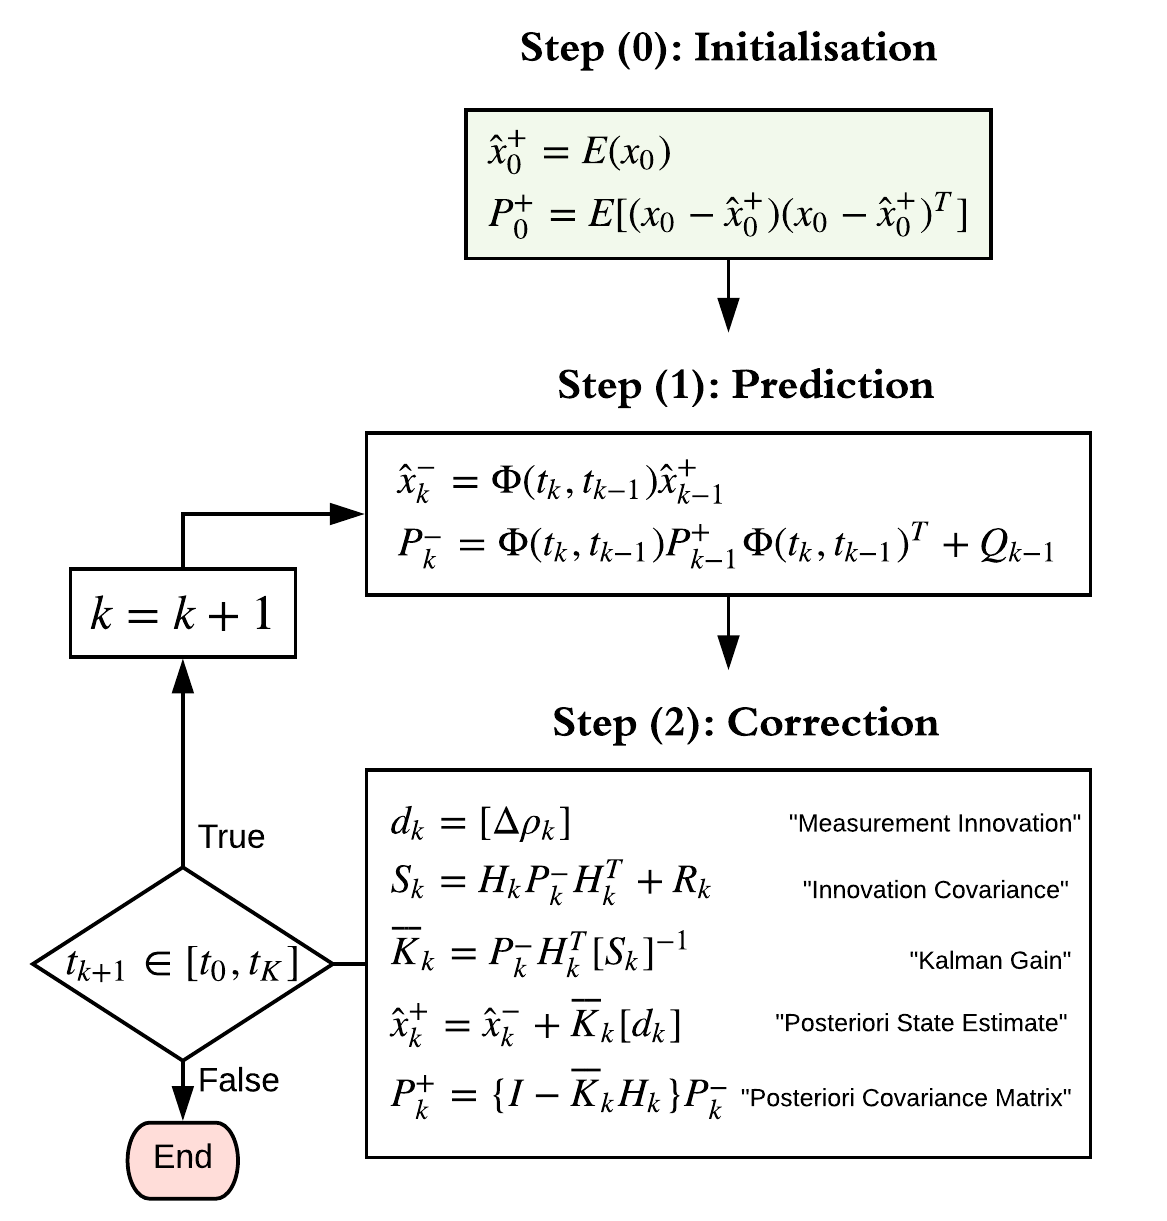
\includegraphics[width=0.55\linewidth]{graphics/CEKF.png}
%    \caption{CEKF flow diagram for process of tracking and data prediction including all equations \cite{3}.}
%    \label{fig:CEKF}
%\end{figure}
%
%
%\begin{figure}[htp]
%    \centering
%    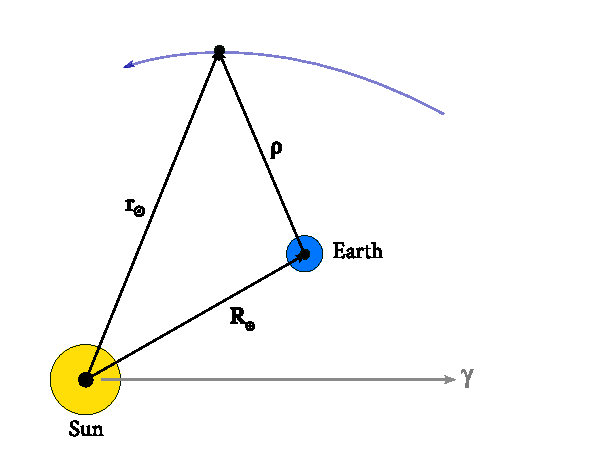
\includegraphics[width=0.5\linewidth]{graphics/pod-1.pdf}
%    \caption{Orbit determination of asteroid using range observations from Earth ($\rho$).}
%    \label{fig:my_label}
%\end{figure}
